% Options for packages loaded elsewhere
\PassOptionsToPackage{unicode}{hyperref}
\PassOptionsToPackage{hyphens}{url}
%
\documentclass[
]{article}
\usepackage{amsmath,amssymb}
\usepackage{lmodern}
\usepackage{iftex}
\ifPDFTeX
  \usepackage[T1]{fontenc}
  \usepackage[utf8]{inputenc}
  \usepackage{textcomp} % provide euro and other symbols
\else % if luatex or xetex
  \usepackage{unicode-math}
  \defaultfontfeatures{Scale=MatchLowercase}
  \defaultfontfeatures[\rmfamily]{Ligatures=TeX,Scale=1}
\fi
% Use upquote if available, for straight quotes in verbatim environments
\IfFileExists{upquote.sty}{\usepackage{upquote}}{}
\IfFileExists{microtype.sty}{% use microtype if available
  \usepackage[]{microtype}
  \UseMicrotypeSet[protrusion]{basicmath} % disable protrusion for tt fonts
}{}
\makeatletter
\@ifundefined{KOMAClassName}{% if non-KOMA class
  \IfFileExists{parskip.sty}{%
    \usepackage{parskip}
  }{% else
    \setlength{\parindent}{0pt}
    \setlength{\parskip}{6pt plus 2pt minus 1pt}}
}{% if KOMA class
  \KOMAoptions{parskip=half}}
\makeatother
\usepackage{xcolor}
\usepackage[margin=1in]{geometry}
\usepackage{graphicx}
\makeatletter
\def\maxwidth{\ifdim\Gin@nat@width>\linewidth\linewidth\else\Gin@nat@width\fi}
\def\maxheight{\ifdim\Gin@nat@height>\textheight\textheight\else\Gin@nat@height\fi}
\makeatother
% Scale images if necessary, so that they will not overflow the page
% margins by default, and it is still possible to overwrite the defaults
% using explicit options in \includegraphics[width, height, ...]{}
\setkeys{Gin}{width=\maxwidth,height=\maxheight,keepaspectratio}
% Set default figure placement to htbp
\makeatletter
\def\fps@figure{htbp}
\makeatother
\setlength{\emergencystretch}{3em} % prevent overfull lines
\providecommand{\tightlist}{%
  \setlength{\itemsep}{0pt}\setlength{\parskip}{0pt}}
\setcounter{secnumdepth}{-\maxdimen} % remove section numbering
\newlength{\cslhangindent}
\setlength{\cslhangindent}{1.5em}
\newlength{\csllabelwidth}
\setlength{\csllabelwidth}{3em}
\newlength{\cslentryspacingunit} % times entry-spacing
\setlength{\cslentryspacingunit}{\parskip}
\newenvironment{CSLReferences}[2] % #1 hanging-ident, #2 entry spacing
 {% don't indent paragraphs
  \setlength{\parindent}{0pt}
  % turn on hanging indent if param 1 is 1
  \ifodd #1
  \let\oldpar\par
  \def\par{\hangindent=\cslhangindent\oldpar}
  \fi
  % set entry spacing
  \setlength{\parskip}{#2\cslentryspacingunit}
 }%
 {}
\usepackage{calc}
\newcommand{\CSLBlock}[1]{#1\hfill\break}
\newcommand{\CSLLeftMargin}[1]{\parbox[t]{\csllabelwidth}{#1}}
\newcommand{\CSLRightInline}[1]{\parbox[t]{\linewidth - \csllabelwidth}{#1}\break}
\newcommand{\CSLIndent}[1]{\hspace{\cslhangindent}#1}
\usepackage[width=\textwidth]{caption}
\usepackage{wrapfig}
\ifLuaTeX
  \usepackage{selnolig}  % disable illegal ligatures
\fi
\IfFileExists{bookmark.sty}{\usepackage{bookmark}}{\usepackage{hyperref}}
\IfFileExists{xurl.sty}{\usepackage{xurl}}{} % add URL line breaks if available
\urlstyle{same} % disable monospaced font for URLs
\hypersetup{
  pdftitle={Floristic Quality Index},
  hidelinks,
  pdfcreator={LaTeX via pandoc}}

\title{Floristic Quality Index}
\author{}
\date{\vspace{-2.5em}}

\begin{document}
\maketitle

\vspace{-1cm}

Floristic Quality Assessments (FQA) utilize the presence of vascular
plant species in an area as indicators of the quality of the habitat.
The fundamental assumption guiding the use of plants as indicators of
habitat quality is that different species respond differently to the
types and frequencies of disturbance. At one end of this spectrum are
species which are able to persist, or may introduced to an area, after
certain types of disturbance - e.g.~compaction of soil via heavy
vehicles. On the other end of the spectrum are taxa which may only grow
in areas which receive episodic disturbances characteristic of their
ecosystem - e.g.~a 100 year flood in a wetland. The subjectively
estimated likelihood of a species either persisting, or being removed
from a site due to disturbance is expressed as a Conservatism Value
(C-Value). C-Values range from 1 to 10 for plants native to North
America, and 0 for plants introduced to the continent by since
colonization by European Settlers, with highly disturbance tolerant
plants being at the upper end of the spectrum.

The use of FQI are uncommon in the Bureau of Land Management, perhaps in
part due to the FQI originating in the Midwest in, and the assignment of
C-values being a task which requires considerable amounts of human
resources (Spyreas
(\protect\hyperlink{ref-spyreas2019floristic}{2019})). A further
requirement which hampers the utilization of these metrics are that each
individual plant species, often times including subspecies, is assigned
a separate C-value, the number of land management professionals which
are capable of distinguishing taxa at these resolutions are limited
(Kramer \& Havens (\protect\hyperlink{ref-kramer2015report}{2015}),
Ahrends et al. (\protect\hyperlink{ref-ahrends2011conservation}{2011}),
Morrison (\protect\hyperlink{ref-morrison2016observer}{2016})). Other
possible limiting factors are that the FQI indices have been
traditionally associated with the portions of Natural Resources focused
on designation of parcels for conservation and preservation, rather than
land management.

While C-values exist for virtually all states East of the Continental
Divide, Colorado is one of only two states with significant surface
lands administered by the BLM which has existing C-values for every
documented member of it's flora (Spyreas
(\protect\hyperlink{ref-spyreas2019floristic}{2019})); additionally BLM
Colorado staff, including the lead state botanist, assisted in
developing these scores (Smith et al.
(\protect\hyperlink{ref-cnhp2020fqi}{2020})). Here we utilize C-values,
to supplement our formal AIM analysis, and to attempt to develop a map
of the habitat quality of the UFO field office.

The Floristic Quality (FQ) Assessments are comprised of two core indices
Mean Coefficient of Conservatism (Mean C) and Floristic Quality Index
(FQI) (see Appendix A for equations). While many novel permutations of
these calculations exist, they seem to offer little insight in addition
to the pair of main indices and appear only useful for niche
applications (Spyreas
(\protect\hyperlink{ref-spyreas2019floristic}{2019})). As the general
goal of the FQA is the assessment of parcels of land, the location of
study areas across different habitat types is accepted, and as we used a
weighted stratified sample design our points meet the assumptions
implicit in the FQA sample design (CITE, Spyreas
(\protect\hyperlink{ref-spyreas2019floristic}{2019})). FQ Assessments
have yet to converge on a standardized size for conducting the species
inventory, and while Mean-C is affected by plot size FQI is relatively
robust against small plot size, however the size of the AIM plot has
been shown to be adequate for noting enough species to conduct the
analyses (Spyreas (\protect\hyperlink{ref-spyreas2016scale}{2016})). In
several applications C-values have been shown to be stable across
sampling time, in part perhaps due to a propensity for many species at a
site to share the same C-values (Spyreas
(\protect\hyperlink{ref-spyreas2016scale}{2016}), Matthews et al.
(\protect\hyperlink{ref-matthews2015null}{2015}), Bried et al.
(\protect\hyperlink{ref-bried2013floristic}{2013})). C-values have also
been shown capable of distinguishing habitat variability more
effectively than the traditional diversity metrics (Taft et al.
(\protect\hyperlink{ref-taft2006estimating}{2006})). Practicioners of
varying degrees of skill are likely to have minimal effects on the
estimates of the FQA indices due to the species encoding some degrees of
redundant information (Bried et al.
(\protect\hyperlink{ref-bried2018experts}{2018}), Spyreas
(\protect\hyperlink{ref-spyreas2019floristic}{2019})).

Utility and Limitations of FQA

FQA scores are tied to the regional list of C-values, accordingly they
cannot be compared across these regions, in other words the FQA scores
of sites in the mixed grass prairies of Kansas and Colorado are
incomparable. Scores have the potential to be misleading if compared
across major habitats, (e.g.~comparing sagebrush steppe to Salt desert).
The score is relatively boundless, e.g.~we could visit plots which we
designate high quality and use them as benchmark for FQI values, but we
cannot incorporate metrics e.g.~land \textgreater{} 4 is `good', until
we consider these locally relevant measurements.

\begin{quote}
\emph{`\ldots{} tolerance of anthropogenic disturbance and exclusivity
to remnant habitats are the only validated criteria for defining FQA.'}
\hfill --- Spyreas 2019
\end{quote}

\begin{quote}
\emph{``\ldots FQA conveys two things about high conservative species:
(1) All else being equal, they have greater conservation value, and (2)
they reflect a site's history of minimal disturbance and degradation.''}
\hfill --- Spyreas 2019
\end{quote}

\hypertarget{methods}{%
\section{Methods}\label{methods}}

Cleaned AIM species richness data were imported from TerrAdat and joined
to the CNHP c-values using the lookup keys developed for the Functional
Diversity section. All species from the plot based species richness
which were not unamibgiously identified to terminal taxon were droppped
from analysis. The Mean Coefficient of Conservatism and Floristic
Quality Index were calculated via the formulation in the appendix. To
determine whether their were bias in the MCoC values between the strata,
a linear model with a single set categorical predictors and a single
continuous response (an `ANOVA'; Analysis of Variance) was used, with a
Kruskall-Wallis Post-hoc test with 95\% Confidence Intervals. The strata
used for detecting differences were those developed in SECTION XXX.

Estimates of the total portion of each parcel of BLM land's condition at
certain Mean COC values were calculated using the `cont\_analysis'
function from spsurvey. This function was used due to BLM not having
metrics of benchmarks, nor what constitutes land meeting them for FQA.

The floristic quality index data are independent of the ecological
sites. Accordingly, we can create a statistical using the plots which
were sampled, and predict the values of floristic quality across the
field office. Based on the map above, and our field experience
collecting these data, we suspected that the variables which are most
related to the FQI scores, and which we could readily acquire or create
were: 1) distance to nearrest road, 2) patch size of federal public
lands, 3) the human population density within \textasciitilde{} 10 km
(\textasciitilde6 miles), 4) elevation. These analyses occurred across
the extent of the mapped area in Figure 1), at a resolution of 90meters.
To calculate the distance of each 90m pixel of BLM land from the nearest
road, the U.S. Census Bureau's `roads' data set was acquired through
`tigris' and simplified using st\_simplify, the distance function of
`terra' was then used to calculate the distances to nearest roads. The
tigris dataset contains nearly all of `major' dirt and gravel roads
across the field office, included many used for historic mining
activities. To calculate the patch size of federal lands, i.e.~all area,
across BLM Forest Service and National Park Service managements, were
queried from the PAD-US database and then these areas were erased using
the tigris road dataset, the areas of each parcel were then calculated
using st\_area from sf, and then converted from meters squared to
hectares, the patches were then converted into a raster using
`rasterize' from terra. To create estimates of population density within
a distance of each pixel of BLM Land, population density data at 30m
resolution were downloaded from HDX (cite). Elevation data were acquired
from EarthEnv, and were prepared by JETZ ET AL. All data sets were
cropped and re-sampled to a template to ensure optimal matching of
cells.

In order to detect variables which were collinear, and hence would
violate assumptions, of independence variance inflation factors
calculated used from the `function' vifstep in the package usdm with a
theta cut off 10 using 5000 random pixels regularly dispersed across the
extent of the sample area (Naimi et al.
(\protect\hyperlink{ref-naimi2014usdm}{2014})). No combination of
variables were suggested to be removed from the analysis, but
collinearity existed between the elevation and x coordinates, this
likely due to the increase in elevation from the Colorado Plateau into
the Rocky Mountains. In order to create a model which could capture the
variation in our data and generalize them, a maximal model of the term
\emph{glm(mcoc\_r \textasciitilde{} road\_dist * pop\_density *
patch\_size * elevation * xcoord * ycoord)} was created. This model was
then fed into the `dredge' function from the package MuMIn, which
creates all smaller models, and evaluates them in an information
theoretic framework (Bartoń
(\protect\hyperlink{ref-Barton2022mumin}{2022})). All tops models, those
with dAIC \textless{} 2.0, were each selected for further analyses; the
combined maximal model for the top terms was: \textasciitilde, mcoc\_r,
elevation + patch\_size + pop\_density + road\_dist. Each model was
checked for the effect of spatial autocorrelation in the residuals by
creating identifying neighboring points using `graph2nb' from and
converting them into three neighbor lists using `nb2listw' (both
functions from `spdep'), the Moran's Index for each model was very low,
despite the Moran's Index for the predictor variables being very high
and showing significant clustering (Bivand
(\protect\hyperlink{ref-bivand2022spdep}{2022})). Subsequent to the
interpretation of the maps produced by the stacked model outputs, and
considering that the model including the coordinates, did not suffer
from autocorrelation, and that the X coordinate was often selected as a
predictor in top models, we believe that collinearity between the X
coordinate and the strongest predictor Elevation indicated that it was
redundant. Accordingly both coordinate terms were removed and a new a
full model in the form \emph{glm(mcoc\_r \textasciitilde{} road\_dist *
pop\_density * patch\_size * elevation)} was passed to MuMIn. The
results of the tops models, those with dAIC \textless= 2.13 were checked
for spatial autocorrelation, using the same methods as the models above.
The general rule of thumb for only utilzing models with dAIC \textless{}
2, was bent in order to accommodate two more models which incorporated
terms we have observed to be ecologically relevant, and are well
supported in the primary literature. After evaluation of the stacked
prediction map from these top models, it was used for the final
analysis, in part because removal of the x-coordinates made it more easy
to interpret, and it was able to utilize the other predictors which are
known to affect species compositions, both universally and strongly.

All six of these candidate AIC models were predicted into space, and the
weighted means, based on each models weight in a final combination
model, were used to generate a consensus prediction layer (Bartoń
(\protect\hyperlink{ref-Barton2022mumin}{2022}), Dormann et al.
(\protect\hyperlink{ref-dormann2018model}{2018})). The consensus
prediction was then clipped to the extent of UFO BLM administered lands.
Most spatial analyses were performed using terra Hijmans
(\protect\hyperlink{ref-hijman2022terra}{2022}), and sf Pebesma
(\protect\hyperlink{ref-pebesma2018sf}{2018}).

\hypertarget{discussion}{%
\section{Discussion}\label{discussion}}

\begin{wrapfigure}{l}{0.3\textwidth}
  \centering
    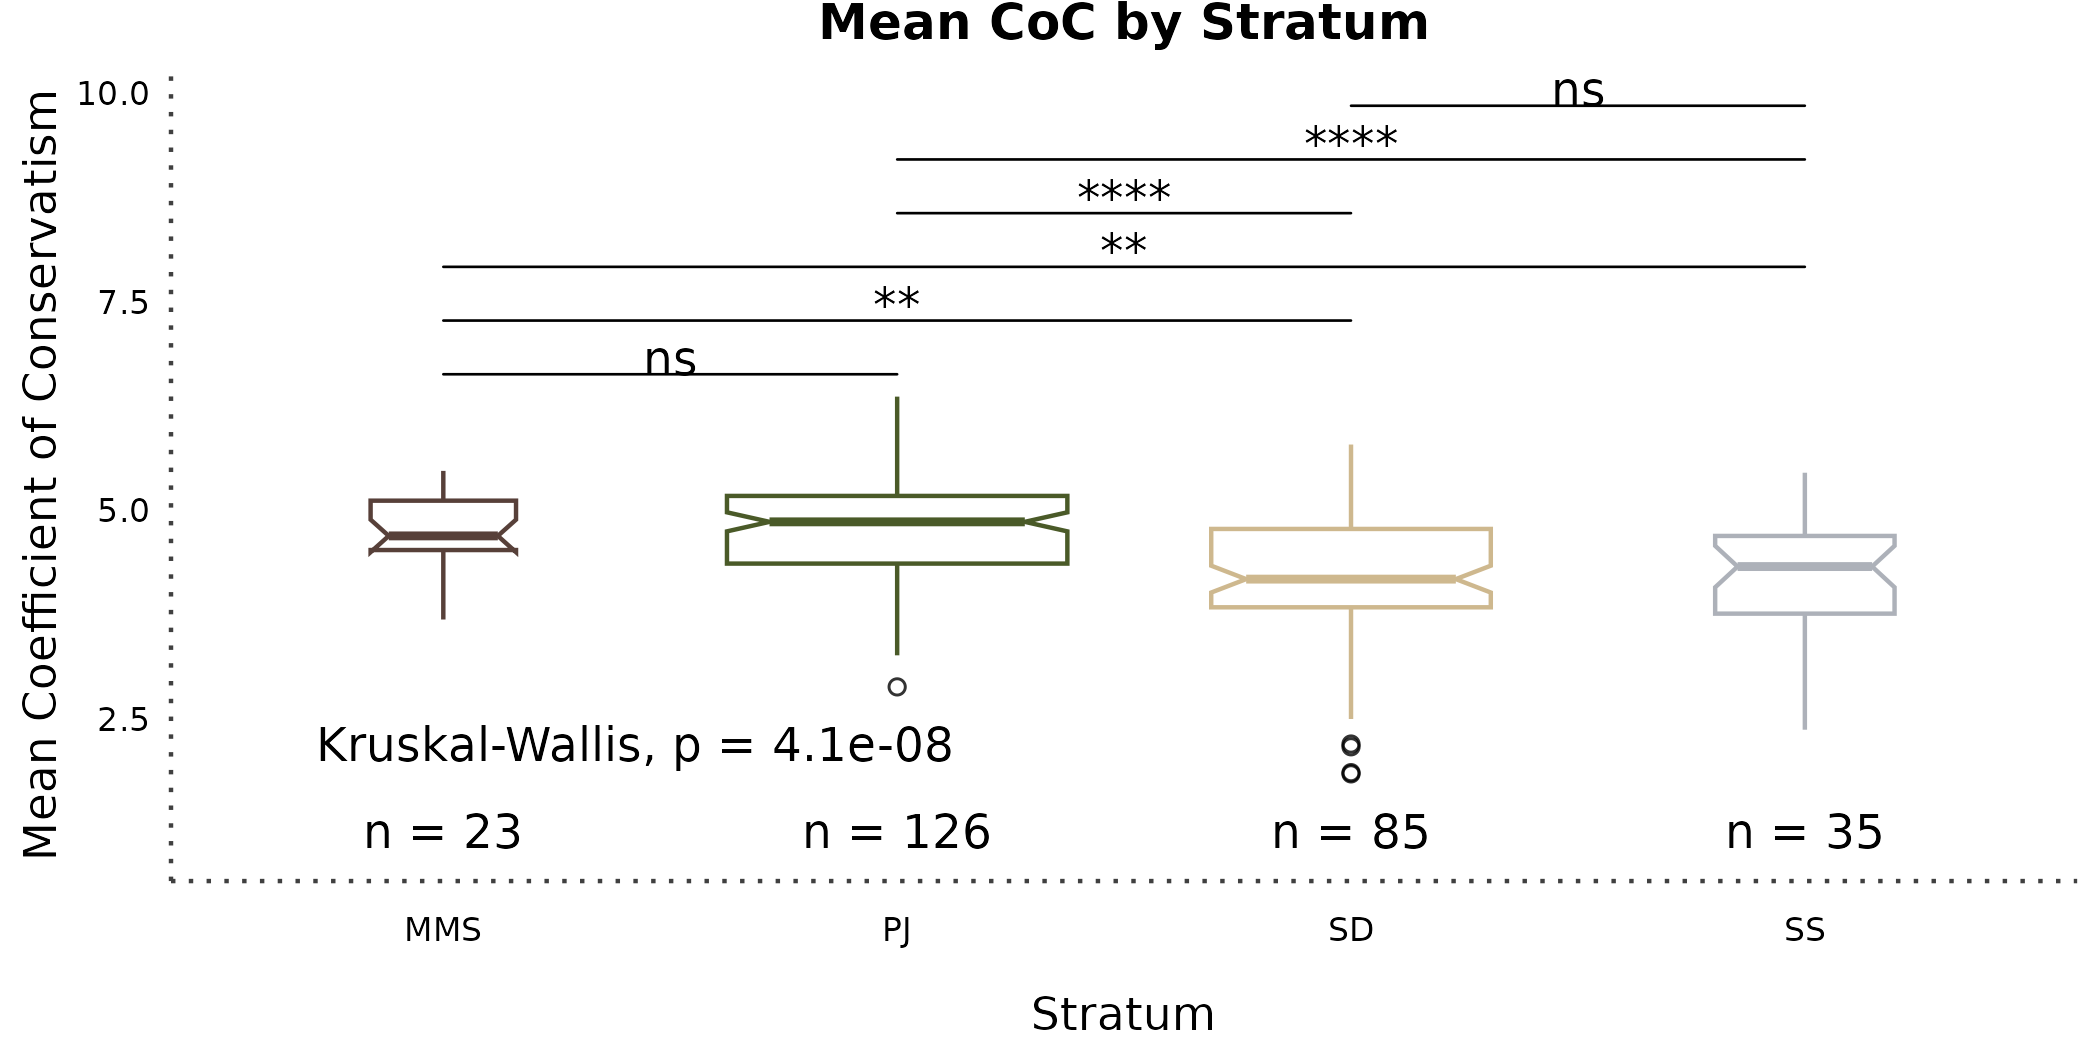
\includegraphics[width=0.3\textwidth]{../plots/graphics/Mcoc_boxplot.png}
  \caption{Comparision of median values by Stratum}
\end{wrapfigure}

The mean C-Values varied by stratum (Analysis of Variance (ANOVA)),
follow-up tests (Kruskall-Wallis) indicated that Salt-Desert and
Sage-Brush sites did not differ from each other, nor Mixed Mountain
Shrub and Pinon-Juniper from each other. Results indicate that all
members of these two groups differed across them, e.g.~Sage-brush
differed from both Mixed Mountain Shrub and Pinon-Juniper and \emph{vice
versa}. The two lower elevation strata, Salt Desert and Sage Brush, are
generally more accessible to humans and have higher recreational land
uses, and had the lowest C-Vals. While the values did vary, the extent
of the variation was minor, with the range of variation from the median
values 4.18 - 4.86 and a mean range of 4.21 - 4.76, given that the these
values occur over a range of 0-10, we considered this to be a negligible
difference, not indicative of major biases in the C-values ascribed to
plants themselves, but rather indicative of actual land conditions.

The generalized linear models were used to predict the floristic quality
of un-sampled areas of BLM Land. Based on AIC model selection a total of
6 top models were retained, and these were then combined into a single
model, of which the weights used to make an ensembled prediction of the
Mean Coefficient of Conservatism. The results from these top models
indicate that all predictors, elevation, human population density,
Federal lands patch size, and distance to nearest road, affect the FQI,
but that by far the strongest predictor is elevation. Elevation was such
a useful predictor, that under certain statistical paradigms our models
may be simplified to include it as the only predictor, and still give
very good results. The other predictors had the expected effect on FQI
as expected, FQI slowly increases as nearby human population density
decreases, and FQI slowly increases as the size of the patch of natural
lands and the distance from the nearest road increase.

From the predicted FQI values we can infer that habitat quality varies
across the field office. In general, the lowest elevation sites display
the lowest values of FQI and Mean CoC. This is especially apparent as
one would be travelling to Montrose from Grand Junction on Highway 50,
before reaching Delta. In particular, these and several other areas of
Salt Desert along Highway 50, and near Crawford are areas of concern.
However, not all Salt Desert is inherently in this condition as can be
seen from the values for a moderately sized parcel of BLM Land
immediately Southeast of Montrose; indicating that human uses of theses
areas may be causal factors in these low values. These areas represent
targets for eventual restoration action. The highest elevation portions
of BLM Land are in the best habitat condition, and very good conditions
range into Pinon-Juniper, including most of the disturbed areas around
historic mining in the West End. By these metrics considerable portions
of BLM Sagebrush areas, such as `Crawford Country' are also in good
condition, given the high priority nature of these areas for Gunnison
Sage Grouse conservation this is promising.

Subjective interpretation suggests these results seem very similar to
those generated by the much more time intensive comparison of Ecological
Sites to Benchmarks. This relationships considers serious consideration
in the use of FQA as a proxy of site condition.

\begin{figure}

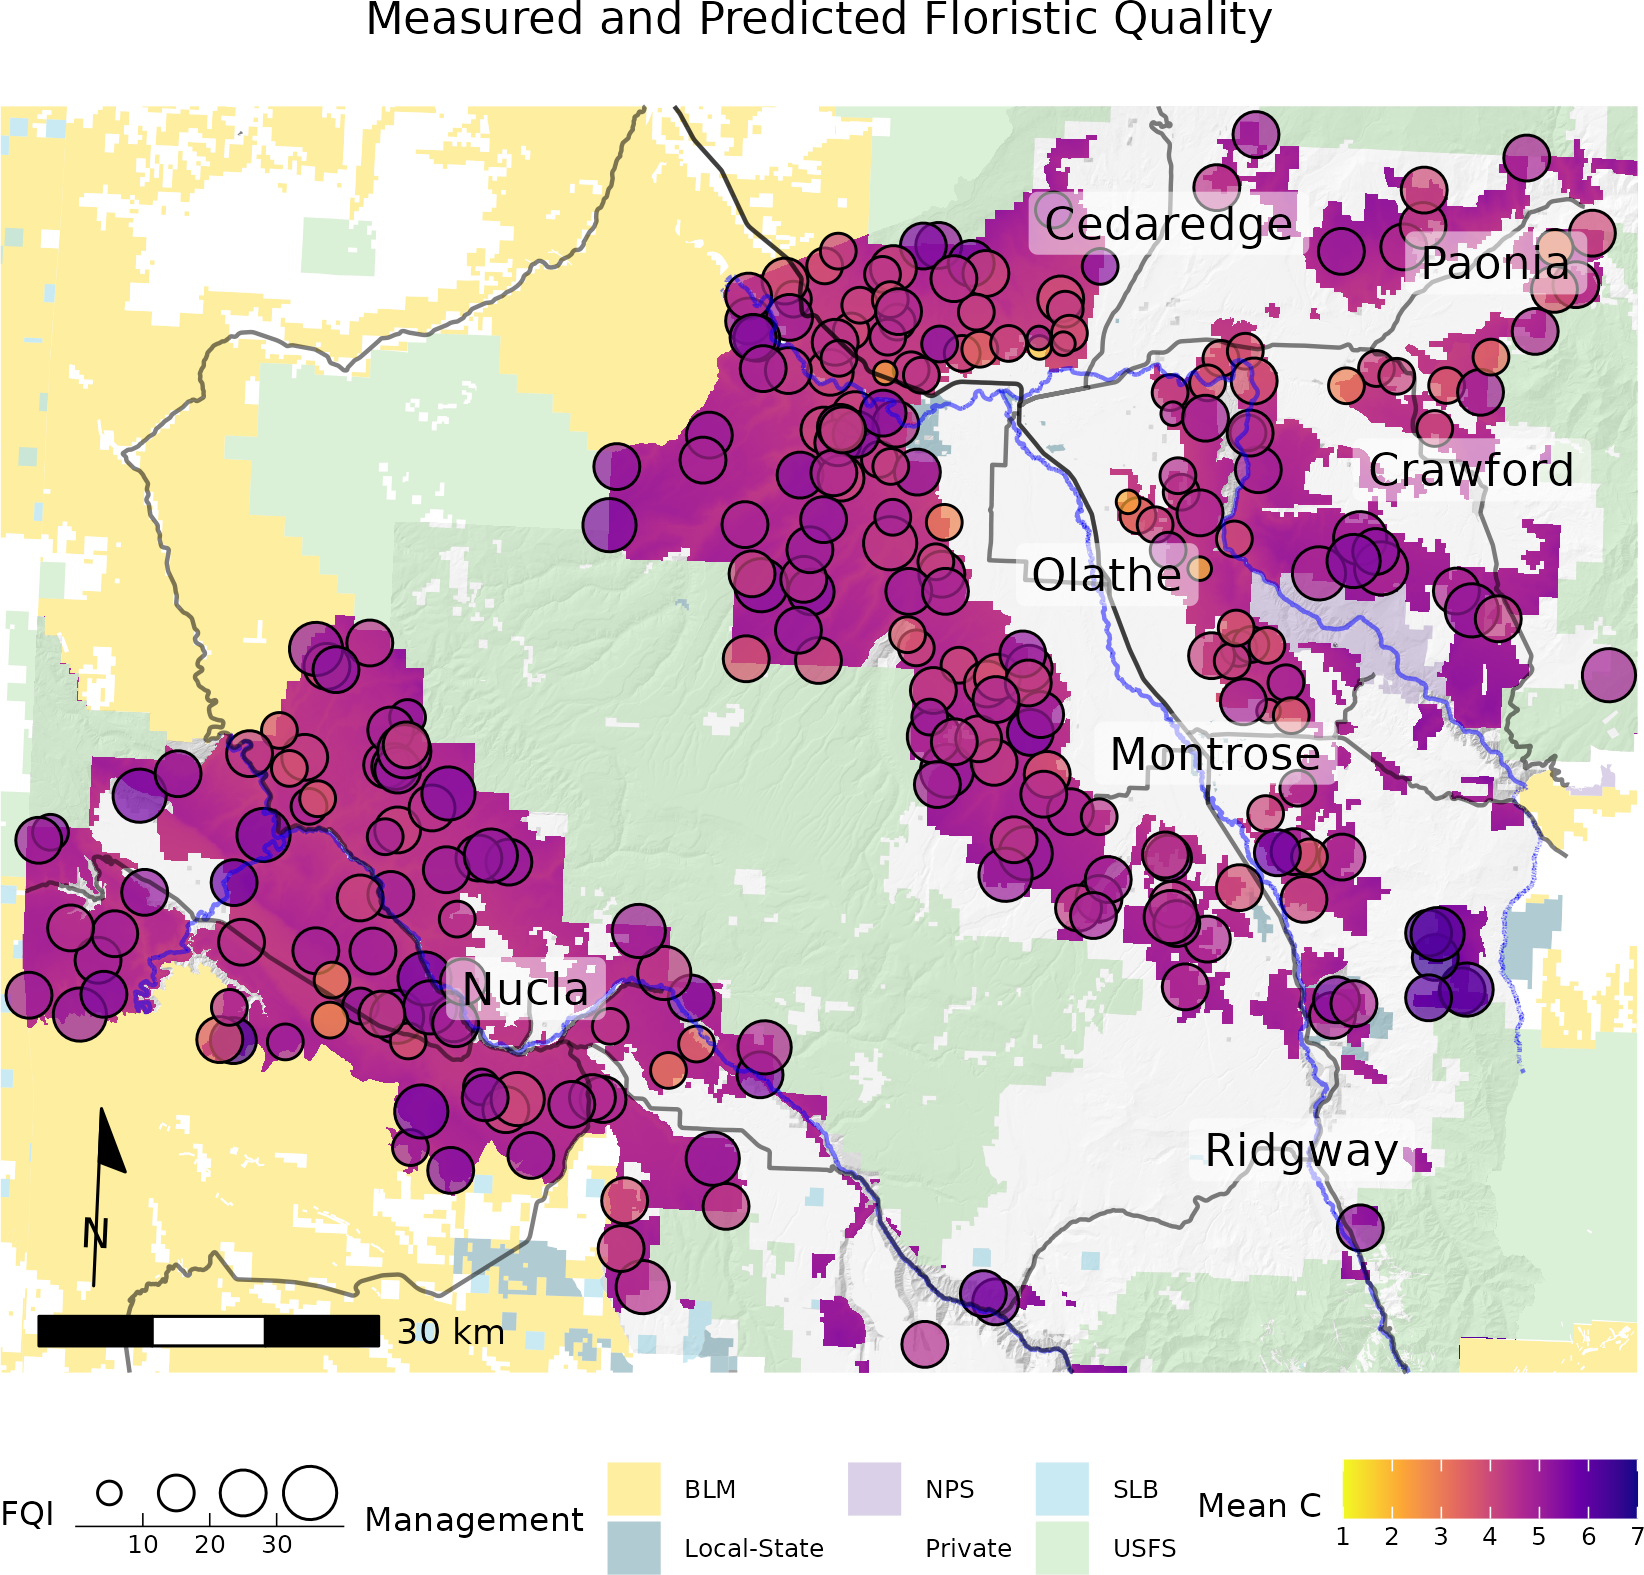
\includegraphics[width=0.95\linewidth]{../plots/maps/FQI} \hfill{}

\caption{Consensus predictions of FQI Values across the UFO Field Office (excluding lands East of Paonia towards Marble)}\label{fig:Map results}
\end{figure}

\newpage

\hypertarget{appendix-a---indices}{%
\subsection{Appendix A - Indices}\label{appendix-a---indices}}

\strut \\
\strut \\
\strut \\

\textbf{Mean Coefficient of Conservatism} \\

\[
\overline{C} = \frac{\sum{} C_i}{S}
\]

Where:\\

\begin{enumerate}[nosep]
  \item[] $\overline{C}$ is the Mean Coefficient of Conservatism, or for short Mean C
  \item[] $S$ is the number of species included in the calculation  
  \item[] $C_i$ in particular $C$ is the Conservatism Value (C-Value), for each $_i$ of the $S$ at the site  
  \item[] $\sum{}$ is an operator, meaning that we will calculate the sum of all C-Values, $C$  
\end{enumerate}

\strut \\
\strut \\
\strut \\
\strut \\
\strut \\
\strut \\
\strut \\

\textbf{Floristic Quality Index} \\

\[
FQI = \overline{C} * \sqrt{S}
\]

Where:\\

\begin{enumerate}[nosep]
  \item[] $\overline{C}$ is the Mean Coefficient of Conservatism, or for short Mean C  
  \item[] $\sqrt{S}$ is the square root of the number of species included in the calculation  
\end{enumerate}

\strut \\
\strut \\
\strut \\
\strut \\
\strut \\
\strut \\
\strut \\

Equations from Swink et al.
(\protect\hyperlink{ref-swink1994plants}{1994}), and modified for
simpler formulations.

\newpage

\hypertarget{references}{%
\section*{References}\label{references}}
\addcontentsline{toc}{section}{References}

\hypertarget{refs}{}
\begin{CSLReferences}{1}{0}
\leavevmode\vadjust pre{\hypertarget{ref-ahrends2011conservation}{}}%
Ahrends, A., Rahbek, C., Bulling, M. T., Burgess, N. D., Platts, P. J.,
Lovett, J. C., Kindemba, V. W., Owen, N., Sallu, A. N., Marshall, A. R.,
et al. (2011). Conservation and the botanist effect. \emph{Biological
Conservation}, \emph{144}(1), 131--140.

\leavevmode\vadjust pre{\hypertarget{ref-Barton2022mumin}{}}%
Bartoń, K. (2022). \emph{MuMIn: Multi-model inference}.
\url{https://CRAN.R-project.org/package=MuMIn}

\leavevmode\vadjust pre{\hypertarget{ref-bivand2022spdep}{}}%
Bivand, R. (2022). R packages for analyzing spatial data: A comparative
case study with areal data. \emph{Geographical Analysis}, \emph{54}(3),
488--518. \url{https://doi.org/10.1111/gean.12319}

\leavevmode\vadjust pre{\hypertarget{ref-bried2018experts}{}}%
Bried, J. T., Allen, B. E., Azeria, E. T., Crisfield, V. E., \& Wilson,
M. J. (2018). Experts and models can agree on species sensitivity values
for conservation assessments. \emph{Biological Conservation},
\emph{225}, 222--228.

\leavevmode\vadjust pre{\hypertarget{ref-bried2013floristic}{}}%
Bried, J. T., Jog, S. K., \& Matthews, J. W. (2013). Floristic quality
assessment signals human disturbance over natural variability in a
wetland system. \emph{Ecological Indicators}, \emph{34}, 260--267.

\leavevmode\vadjust pre{\hypertarget{ref-dormann2018model}{}}%
Dormann, C. F., Calabrese, J. M., Guillera-Arroita, G., Matechou, E.,
Bahn, V., Bartoń, K., Beale, C. M., Ciuti, S., Elith, J., Gerstner, K.,
et al. (2018). Model averaging in ecology: A review of bayesian,
information-theoretic, and tactical approaches for predictive inference.
\emph{Ecological Monographs}, \emph{88}(4), 485--504.

\leavevmode\vadjust pre{\hypertarget{ref-hijman2022terra}{}}%
Hijmans, R. J. (2022). \emph{Terra: Spatial data analysis}.
\url{https://CRAN.R-project.org/package=terra}

\leavevmode\vadjust pre{\hypertarget{ref-kramer2015report}{}}%
Kramer, A. T., \& Havens, K. (2015). Report in brief: Assessing
botanical capacity to address grand challenges in the united states.
\emph{Natural Areas Journal}, \emph{35}(1), 83--89.

\leavevmode\vadjust pre{\hypertarget{ref-matthews2015null}{}}%
Matthews, J. W., Spyreas, G., \& Long, C. M. (2015). A null model test
of floristic quality assessment: Are plant species' coefficients of
conservatism valid? \emph{Ecological Indicators}, \emph{52}, 1--7.

\leavevmode\vadjust pre{\hypertarget{ref-morrison2016observer}{}}%
Morrison, L. W. (2016). Observer error in vegetation surveys: A review.
\emph{Journal of Plant Ecology}, \emph{9}(4), 367--379.

\leavevmode\vadjust pre{\hypertarget{ref-naimi2014usdm}{}}%
Naimi, B., Hamm, N. a.s., Groen, T. A., Skidmore, A. K., \& Toxopeus, A.
G. (2014). Where is positional uncertainty a problem for species
distribution modelling. \emph{Ecography}, \emph{37}, 191--203.
\url{https://doi.org/10.1111/j.1600-0587.2013.00205.x}

\leavevmode\vadjust pre{\hypertarget{ref-pebesma2018sf}{}}%
Pebesma, E. (2018). {Simple Features for R: Standardized Support for
Spatial Vector Data}. \emph{{The R Journal}}, \emph{10}(1), 439--446.
\url{https://doi.org/10.32614/RJ-2018-009}

\leavevmode\vadjust pre{\hypertarget{ref-cnhp2020fqi}{}}%
Smith, P., Doyle, Georgia, \& Lemly, J. (2020). \emph{Revision of
colorado's floristic quality assessment indices}. Colorado Natural
Heritage Program.
\url{https://cnhp.colostate.edu/download/documents/2020/CO_FQA_2020_Final_Report.pdf}

\leavevmode\vadjust pre{\hypertarget{ref-spyreas2016scale}{}}%
Spyreas, G. (2016). Scale and sampling effects on floristic quality.
\emph{PloS One}, \emph{11}(8), e0160693.

\leavevmode\vadjust pre{\hypertarget{ref-spyreas2019floristic}{}}%
Spyreas, G. (2019). Floristic quality assessment: A critique, a defense,
and a primer. \emph{Ecosphere}, \emph{10}(8), e02825.

\leavevmode\vadjust pre{\hypertarget{ref-swink1994plants}{}}%
Swink, F., Wilhelm, G., et al. (1994). \emph{Plants of the chicago
region}. Indiana Academy of Science.

\leavevmode\vadjust pre{\hypertarget{ref-taft2006estimating}{}}%
Taft, J. B., Hauser, C., \& Robertson, K. R. (2006). Estimating
floristic integrity in tallgrass prairie. \emph{Biological
Conservation}, \emph{131}(1), 42--51.

\end{CSLReferences}

\end{document}
